\section{Dataset and Experimental Setup}
As mentioned earlier, this paper based its evaluation of CNN for natural
environment on a particular dataset we have been creating since August 2013.
Since then, every 8 to 15 days, we operate an autonomous surface vessel
(Kingfisher from Clearpath Robotics, see fig.~\ref{fig:kingfisher}) around a small lake next to our campus.
This lake is 400m long by 200m wide, with a small island and a total perimeter
of 1km. Its shores are covered with trees, from small bushes to tall full-grown
trees, some at the water line, others further away, grass areas are mixed
with the shrubberies and a small scenic trail runs around the lake. Some of the
places (as in fig.~\ref{fig:dataset-hard}) have office buildings in the
background. 
\begin{figure}[htb]
    \centering
    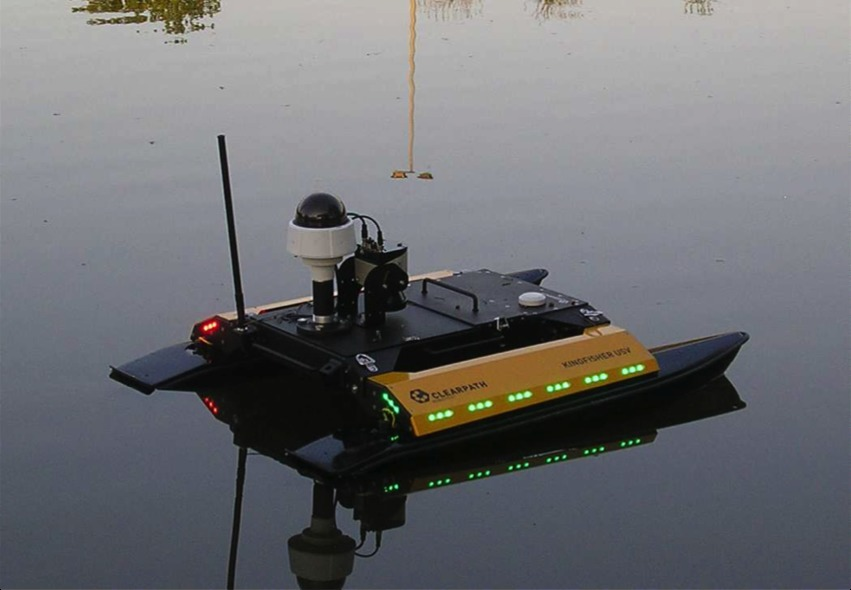
\includegraphics[width=0.4\textwidth]{images/kingfisher}
    \caption{The Kingfisher on a very smooth lake. The pan-tilt camera is
        housed in the white dome at the back of the boat, just behind the laser
    scanner used for navigation.}
    \label{fig:kingfisher}
\end{figure}

Every survey we collect contains images acquired by a pan-tilt surveillance
camera ($704\times480$ pixels) at 10Hz with a slight JPEG compression. The boat
runs autonomously at a constant distance of 10m to the shore (lattice-type
local planner) and at a bit less than 1km/h. This means that a survey is a
collection of close to 40'000 images, acquired with the camera pointing to the
port or starboard side of the boat (i.e. $\pm90^o$ from the direction of
travel). In addition to the images, we record all the boat sensor data:
position from GPS, heading from compass, pitch and roll angle from IMU although
they can be neglected and proximetry from the laser range finder (not used
beyond the on-board controller in this study). 

In this study, we are considering 80 surveys from the second half of 2013 up to
the end of 2015. This corresponds to potentially a bit more than 3'000'000
images collected over 80km of autonomous navigation. 

The particularity of our dataset is that most of our images depicts natural
scenes combining some water, trees and shrubberies at various distances,
sometimes grass areas and/or far-away buildings, and sky. All of these elements
are challenging for computer vision: the lake surface acts as a somewhat
deformable mirror, sometimes very smooth and reflective and at other times not
reflective at all due to wavelets. Additionally, flooding events means that the
water line can move by up to 1m in some surveys. Trees are challenging for
three reasons, first these ones do not always have leaves, second they are
fractal self-similar structures, and last they are 3D semi-transparent
structures whose appearance is very sensitive to view point, especially in
winter. Finally, the sky varies with the weather and the sun position. Because
we run the boat on the perimeter of the lake at different times of the day and
as long as it is not raining (to avoid water drops on the camera dome), our
images are also sometimes affected by sun-glares or very challenging dynamic
range requirements. 

% Dataset:
% - Environmental images from 2013 to 2015
% - Seasonal changes
% - Lighting changes
% - Video frames from camera XXXXX

